% Options for packages loaded elsewhere
\PassOptionsToPackage{unicode}{hyperref}
\PassOptionsToPackage{hyphens}{url}
%
\documentclass[
]{article}
\usepackage{amsmath,amssymb}
\usepackage{lmodern}
\usepackage{iftex}
\ifPDFTeX
  \usepackage[T1]{fontenc}
  \usepackage[utf8]{inputenc}
  \usepackage{textcomp} % provide euro and other symbols
\else % if luatex or xetex
  \usepackage{unicode-math}
  \defaultfontfeatures{Scale=MatchLowercase}
  \defaultfontfeatures[\rmfamily]{Ligatures=TeX,Scale=1}
\fi
% Use upquote if available, for straight quotes in verbatim environments
\IfFileExists{upquote.sty}{\usepackage{upquote}}{}
\IfFileExists{microtype.sty}{% use microtype if available
  \usepackage[]{microtype}
  \UseMicrotypeSet[protrusion]{basicmath} % disable protrusion for tt fonts
}{}
\makeatletter
\@ifundefined{KOMAClassName}{% if non-KOMA class
  \IfFileExists{parskip.sty}{%
    \usepackage{parskip}
  }{% else
    \setlength{\parindent}{0pt}
    \setlength{\parskip}{6pt plus 2pt minus 1pt}}
}{% if KOMA class
  \KOMAoptions{parskip=half}}
\makeatother
\usepackage{xcolor}
\IfFileExists{xurl.sty}{\usepackage{xurl}}{} % add URL line breaks if available
\IfFileExists{bookmark.sty}{\usepackage{bookmark}}{\usepackage{hyperref}}
\hypersetup{
  pdftitle={Monothetic Clustering with Feature Selection},
  pdfauthor={Paul Harmon},
  hidelinks,
  pdfcreator={LaTeX via pandoc}}
\urlstyle{same} % disable monospaced font for URLs
\usepackage[margin=1in]{geometry}
\usepackage{graphicx}
\makeatletter
\def\maxwidth{\ifdim\Gin@nat@width>\linewidth\linewidth\else\Gin@nat@width\fi}
\def\maxheight{\ifdim\Gin@nat@height>\textheight\textheight\else\Gin@nat@height\fi}
\makeatother
% Scale images if necessary, so that they will not overflow the page
% margins by default, and it is still possible to overwrite the defaults
% using explicit options in \includegraphics[width, height, ...]{}
\setkeys{Gin}{width=\maxwidth,height=\maxheight,keepaspectratio}
% Set default figure placement to htbp
\makeatletter
\def\fps@figure{htbp}
\makeatother
\setlength{\emergencystretch}{3em} % prevent overfull lines
\providecommand{\tightlist}{%
  \setlength{\itemsep}{0pt}\setlength{\parskip}{0pt}}
\setcounter{secnumdepth}{-\maxdimen} % remove section numbering
\usepackage{booktabs}
\usepackage{longtable}
\usepackage{array}
\usepackage{multirow}
\usepackage{wrapfig}
\usepackage{float}
\usepackage{colortbl}
\usepackage{pdflscape}
\usepackage{tabu}
\usepackage{threeparttable}
\usepackage{threeparttablex}
\usepackage[normalem]{ulem}
\usepackage{makecell}
\usepackage{xcolor}
\ifLuaTeX
  \usepackage{selnolig}  % disable illegal ligatures
\fi

\title{Monothetic Clustering with Feature Selection}
\author{Paul Harmon}
\date{4/5/2022}

\begin{document}
\maketitle

\hypertarget{introduction}{%
\section{Introduction}\label{introduction}}

Clustering is an important method for unsupervised statistical learning
that allows for data-driven identification of similar observations or
objects. Consider a data matrix \(X\) with n observations or objects and
p features. Various methods for clustering X into meaningful groups
exist. Clustering has long been a primary tool for data scientists to
determine groups in unsupervised data problems (see Kaufman and
Rousseeuw, 199); Everitt and Hothorn, 2011). When no clear groups are
identified, clustering can be used to identify common characteristics
between observations and to group them into similar groups based either
on single characteristics or on relationships between many
characteristics.

However, in many cases, data may contain many features. Not all of those
features will be likely to contain predictive signal. Sparse clustering
attempts to reduce the number of features used as input in a clustering
problem in order to drive better results, for several reasons. In some
cases, such as high-dimensional settings where the number of
observations \(n\) is less than the number of data features \(p\), some
clustering algorithms will perform poorly or break down completely
(Witten and Tibshirani, 2010). However, the data need not be
high-dimensional to pose potential problems for clustering algorithms;
in many cases, the true number of signal-bearing features may be less
than the total number of features available to be used - these remaining
``noise features'' can actually hamper the ability of the algorithm to
segregate the data into groups that best represent the truth (Brodinova
et al., 2019).

Clustering requires some measure of distance, or dissimilarity, between
pairs of objects. In many cases, \(d(x_i,x_j)\) refers to the measure of
similarity between objects \(x_i\) and \(x_j\). A common choice for
distance is the squared Euclidean distance across the \(p\) features
\(d(x_i, x_j) = \sum_{j=1}^p (X_{ij} - X_{i'j})^2\). Hierarchical
clustering methods take as input \(D\), the dissimilarity/distance
matrix of all pairwise \(d(x_i,x_j)\) across the \(p\) features. Other
methods, such as K-means or K-medoids, can be applied directly to the
data matrix and take the dissimilarity measure into account as part of
their objective function. In many cases, clustering methods are
considered polythetic, meaning that the clusters can be characterized by
a shared set of variables, or monothetic, meaning that the cluters can
be characterized by at least one well-defined common property.

In clustering, as in many statistics problems, Occam's Razor applies -
the simplest, parsimonious solution tends to provide the best results.
Additionally, for hierarchical methods, a method for linkage must be
defined - this is the way that distances between clusters are defined.
Thus, it is desirable to cluster based only on the signal-bearing
features and dispose of those noise-bearing ones prior to application of
the clustering method. From this idea arises the concept of sparse
clustering posed by Witten and Tibshirani (2010), which breaks the
clustering method into a feature-selection step followed by a clustering
step. Three critical advantages can be obtained by using sparse
clutering methods; chiefly, the solution is more interpretable because
it relies on fewer features and the cluster solution will potentially be
more accurate; additionally, for some methods, removal of noise features
may lead to potentially large improvements in computational performance.

This paper proposes a method for sparse monothetic clustering, which
takes the framework proposed by Witten and Tibshirani (2010) and extends
it to the monothetic clustering method initially presented by Chavent
(1998) and operationalized in the the monoclust package in statistical
software R (Tran, 2019).

\hypertarget{monothetic-clustering}{%
\subsection{Monothetic Clustering}\label{monothetic-clustering}}

Monothetic clustering (Sneath and Sokal, 1973) differs from the above
polythetic hierarchical clustering methods in that it makes decisions
based on a single property at a time; resulting clusters thus share a
set of characteristics rather than simply being ``similar'' based to a
dissimilarity metric that may take several features into account. This
property of monothetic clustering means that the resulting clusters are
easier to interpret, generally, than those created by other hierarchical
clutering methods. Methods for doing monothetic clustering are
overviewed in Tran (2019) and are implemented in the R package monoClust
(Tran, 2021).

Monothetic clustering methods first arose in the case of binary data
(Williams and Lambert, 1959) and have since been known as descendant
conceptual clustering methods (Michalski et al., 1981). A method for
monothetic clustering, inspired partly by the classification and
regression trees of Breiman, et al (1984) was developed by Chavent
(1998). The algorithm performs both a hierarchy of a set of objects (a
recursive clustering) as well as a monothetic characterization of each
cluster (i.e., a common, interpretable characteristic in each group).

A global criterion, called \textit{inertia}, which is defined as the
total variability around the cluster centroid, can be used as a target
for a monothetic clustering algorithm that iteratively searches for
optimal splits from each multivariate response (feature). When the
chosen dissimilarity metric is Euclidean distance, the \textit{inertia}
for cluster \(C_k\) is equivalent to \(I(C_k)\) in Ward's Method as
noted in Equation \ref{eq:wardD}.

Let \(N\) be the number of objects in a set \(\Omega\). Each object is
described on \(p\) features \(Y_1,..., Y_p\), which are weighted equally
(although note that this need not be the case, indeed the interest of
this dissertation is to re-weight the \(Y\)'s in a data-driven fashion).
The \textit{intertia}, denoted \(I(C_k)\), is a measure of homogeneity
within a cluster defined as: \begin{equation}
    I(C_k) = \frac{1}{n_k}\sum_{i,j \in C_k, i>j} d^2_{euclidean}(y_i, y_j), 
\end{equation}

where \(n_k\) is the cardinality (i.e., the number of unique
observations) in cluster \(C_k\).

Note that minimizing the within-cluster inertia of a partition (i.e.,
the similarity of objects within each cluster) is equivalent to
maximizing the between-cluster inertia (the dis-similarity of objects in
separate clusters) - this theme of monothetic clustering means that the
method is similar in its goal to both K-means/medoids clustering as well
as hierarchical clustering with Ward's method as the selected linkage.

A binary split \(s(C_k)\) on a given cluster \(C_k\) will result in a
partition of the original cluster into two smaller clusters, \(C_{kL}\)
and \(C_{kR}\) (L and R refer to `left' and `right' in the dendrogram
produced). The inertia decrease before and after the partition is
defined as

\begin{equation}
    \Delta(s,C_k) = I(C_k) - I(C_{kL}) - I(C_{kR}),
\end{equation}

and the optimal split \(s^*(C_k)\) is the one that maximizes this
decrease in inertia. \(s^*(C_k)\) denoted as

\begin{equation}
    s^*(C_k) = argmax_{s} \Delta(s,C_k).
\end{equation}

Various simulation studies have been performed on the monothetic
clustering method proposed by Chavent (1998) as well comparisons to
other clustering methods (Chavent, et al, 2007). Comparing across
simulated datasets as well as six real datasets, they found that the
monothetic clustering algorithm outperformed k-means and Ward's methods
in making correct classifications when the number of clusters was small.
Additionally, in the case of numerical datasets, monothetic clustering
outperformed the other methods when data volumes were higher. Tran
(2019) additionally extended the method to implementations on both
circular variables and the aforementioned functional data settings.

R Package \emph{monoClust} (Tran, 2020) used to generate clusters.

\hypertarget{motivating-example}{%
\subsubsection{Motivating Example}\label{motivating-example}}

Witten and Tibshirani present a motivating example to illustrate why
sparse K-means is useful compared to a K-means method that takes
advantage of all the potential data. Simulating from a multivariate
normal distribution where two groups differ only by a mean shift on the
two features, they demonstrate that K-means as applied to both features
will not result in good group discrimination vs.~K-means applied only to
the axis where the groups are shifted.

Because monothetic clustering makes bipartitions based on a single
feature at a time, in a bivariate case it will either split the data
horizontally or vertically. Thus, the situation proposed by Witten and
Tibshirani (2010) must be modified so that no horizontal or vertical
split completely separates the groups. Instead, we consider a
tightly-bound bivariate normal distribution simulated next to a more
variable group simulated with from a bivariate normal with both shifted
mean and variance.

As shown in Figure XX, the actual cluters are not completely separated,
nor can they be separated with a single vertical or horizontal line.
Monothetic clustering as applied to both features simultaneously
provides a curiously un-intuitive result, splitting based on V2, the
feature on the Y-axis and yielding a Rand Index of 0.86. By using only
the first feature, V1, the ``sparse'' monothetic clustering method is
able to find a more intutive bipartition with a much higher Rand Index
of 0.97. In such a case, a sparse monothetic method not only better
captures the cluter membership but also more useful monothetic
characterization of the data based on the more signal-bearing variable,
V1. Note that the CER is simply 1-Rand Index, so equivalently, the CER
is lower for the sparse monothetic clutering scenario and higher for the
version that takes both features into account.

\begin{figure}
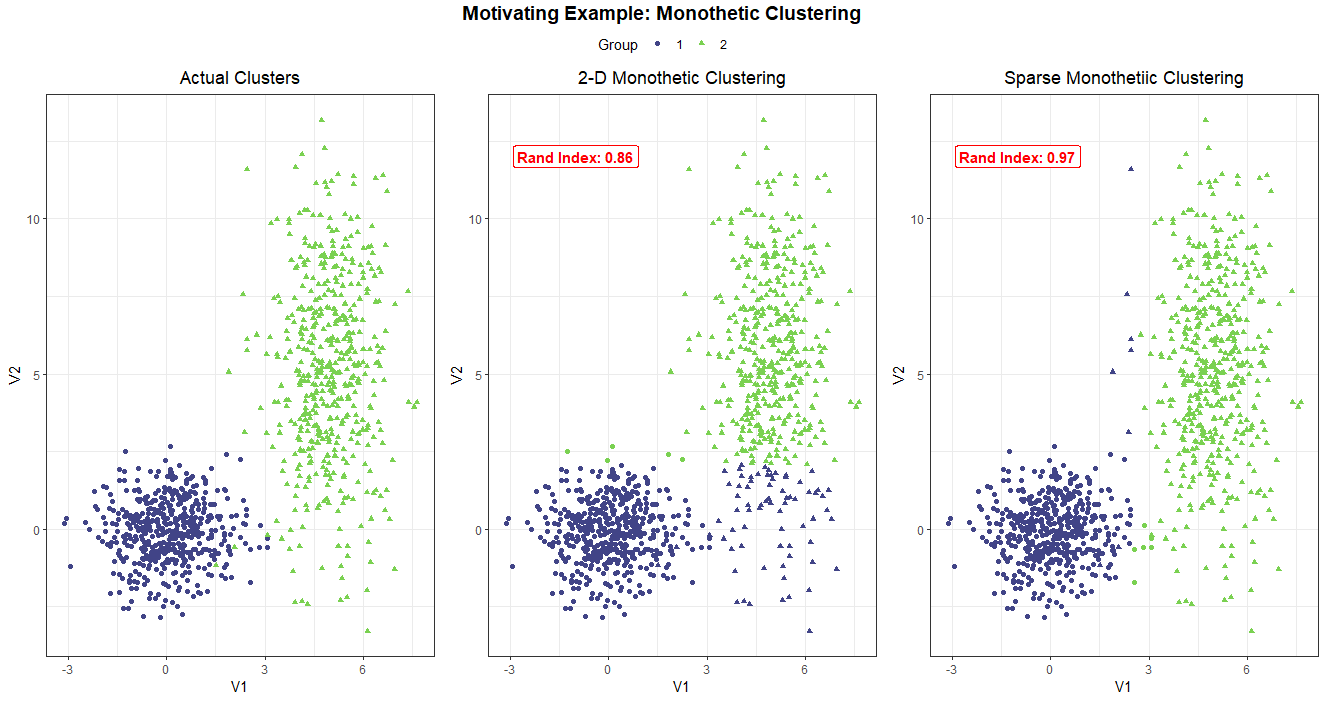
\includegraphics[width=0.9\linewidth]{SparseMotivatingExample} \caption{Motivating Example showing improved monothetic clustering results}\label{fig:MotivatingExample}
\end{figure}

\hypertarget{existing-methods-for-sparse-clustering}{%
\subsection{Existing Methods for Sparse
Clustering}\label{existing-methods-for-sparse-clustering}}

Witten and Tibshirani (2011) introduced a framework for sparse
clustering that is further expounded in Hastie et al (2015). To achieve
sparsity, a two-step method is proposed. First, a matrix decomposition
must be performed to provide either a reweighted distance/dissimilarity
matrix, or a set of weights that can be applied to the original objects
to effectively ``sparsify'' the original data. Then, the reweighted
distance/dissimilarity matrix can be used as a newly sparse input to
methods like Hierarchical Clustering that take the distance matrix as
input. In the case of K-means and methods that can be applied to the
original data, the weights can be more directly applied. In general,
Witten and Tibshirani first pose the sparse clustering problem in the
following form:

\[\underset{(\Theta \in G)}{max} ~ ~ {\sum_{j=1}^{p}w_j f_j(X_j, \Theta)} \]
Subject to three constraints:

\begin{itemize}
\tightlist
\item
  \[ ||w||_2^2 \leq 1 \]
\item
  \[ ||w||_1 |leq s\]
\item
  \[ w_j \geq 0\]
\end{itemize}

In this case, \(w_j\) refer to a set of weights that are applied to each
feature and s is a tuning parameter that, like \(\lambda\) in standard
Lasso regression, controls how sparse the feature set used should be.
This provides a general framework wherein the first constraint, the
squared L2 norm, assures that at least one feature will be nonzero. The
L1 norm provides penalization that allows weights to be shrunk all the
way to 0.

\hypertarget{sparse-k-means-clustering}{%
\subsubsection{Sparse K-Means
Clustering}\label{sparse-k-means-clustering}}

In a K-means setting, this can be directly utilized to optimize the
dimensionality of the space used in the k-means algorithm. A sparse
K-means

Witten and Tibshirani (2010) apply sparsity to clustering via estimation
a Lasso-penalized weighting of the variables \(w_j\) used in
dissimilarity matrix \textbf{D}. We denote the weighted dissimilarity
matrix \(D^*\). The below solution maximizes the between-cluster SS
(BCSS) in K-means:

\[ max_{(C_1,...C_k,w)} \sum_{j=1}^{J}w_j ~ ~[\frac{1}{n}\sum_{i} \sum_{i'} d_{i,i',j} - \sum_{k=1}^{K}\frac{1}{n_k}\sum_{i'i' \in C_k}d_{i,i',j}]\]

subject to \(\|w||_{2}^{2} \leq 1\) and \$
\textbar\textbar w\textbar\textbar\_1 \textless{} s\$.

Where \(s\) is a tuning parameter to control the sparsity and
\(w_j \geq 0 ~ \forall j\)

Much of the research following Witten and Tibshirani has focused on
improvements to the sparse K-Means implementation. Brodinova et
al.~(2019) introduced a framework for dealing with outliers in the
presence of noise features by incorporating a weighting function that
penalizes outlying observations, effectively adding weighting to the
objects to be clustered as well as the features that were already
subject to constraints. Arias-Castro and Pu (2016) propose a slightly
different alternative to Witten and Tibshirani's approach called Sparse
Alternate Sum (SAS) Clustering that is applied to K-medoids, instead
applying a hill-climbing method that is more directly optimized than the
alternating optimization necessary for Sparse K-means.

\hypertarget{sparse-hierarchical-clustering}{%
\subsubsection{Sparse Hierarchical
Clustering}\label{sparse-hierarchical-clustering}}

A direct translation of this framework cannot be applied to hierarchical
clustering in the way that it is applied to k-means clustering, because
hierarchical clustering does not directly optimize a criterion in the
above form. This results because HC generates a dendrogram that provides
a solution for all potential splits from the singleton cluster solution
to the n-cluster solution - these have dendrograms have to be cut at a
certain point to provide a single clustering. Witten and Tibshirani
(2010) make the point that one could attempt to build a sparse
hierarchical clustering algorithm that cuts the dendrogram, calculates
the BCSS that results, and optimizes based on that criterion. However,
such a case would require a more obvious method for when and how to cut
the dendrogram, and this is not a trivial problem.

However, Witten and Tibshirani develop a method that recasts the
dissimilarity matrix \({d_{i,i'}}_{nxn}\) as the solution to the below
optimization:

\[\underset{w, U \in R^{nxn}}{max} \{\sum_{j = 1}^{p}\sum_{i,i'=1}^{n} d_{i,i',j}U_{i,i'}\} \]
Subject to the following constraints:

\begin{itemize}
\tightlist
\item
  \[ \sum_{i,i'=1}^{n} U^2_{i,i'} \leq 1\]
\item
  \[ ||w||_2^2 \leq 1 \]
\item
  \[ ||w||_1 |leq s\]
\item
  \[ w_j \geq 0\]
\end{itemize}

The solution to the optimization uses components of Witten's Sparse
Principal Component (2009) proposal. The algorithm is as follows:

\begin{itemize}
\tightlist
\item
  Let \(u\) be a vector of length \(n^2\) containing all elements in
  \((U_{i,i'})_{nxn}\) strung out
\item
  D (termed dists in code) is \(n^2 x p\) matrix whose jth columns
  contain the \(n^2\) elements of \((d_{i,i',j})_{nxn}\) dissimilarity
  matrix based on the jth feature.
\end{itemize}

This yields:

\[ \underset{w,u}{max} (u^T Dw)\] subject to:

\begin{itemize}
\tightlist
\item
  \[ ||w||_2^2 \leq 1 \]
\item
  \[ ||w||_1 |leq s\]
\item
  \[ ||u||^2_2 \leq 1\]
\end{itemize}

The code calculates these components w and u and iterates until
convergence to get \textbf{both} the optimal weights \(\hat{w}\) and the
vectorized dissimilarity constraint \(\boldsymbol{u}\).

\hypertarget{cosa-alternative}{%
\subsubsection{COSA Alternative}\label{cosa-alternative}}

An alternative to the reweighted distance/dissimilarity matrix provided
by the penalized matrix decomposition of Witten and Tisbhirani (2009)
can be generated using a method called Clustering Objects on Subsets of
Attributes (COSA, Friedman and Muelman, 2004). Motivated by problems in
high-dimensional settings, COSA seeks to accomplish two tasks:
clustering objects into homogenous groups while collecting (potentially
overlapping) subsets of variables for each group of objects.

COSA seeks to solve the following optimization poblem

\[minimize \sum_{k \in K} \alpha(|C^{-1}(k)|) \sum){i,j \in C^{-1}(k)} \sum_{\alpha \in [p]}(w_a d(i,j) + \lambda w_alog(w_a)),\]
over any clustering C and a set of weights \(w_1,...,w_p \geq 0\)
subject to \(\sum_{\alpha \in [p]} w_a = 1\). The \(\alpha\) is defined
as a function that can take on various forms, but when
\(\alpha(u) = \frac{1}{u}\), the objective function can be simply
expressed as

\[\sum_{\alpha \in [p]} (w_a\Delta_a[C] + \lambda w_a log(w_a)).\]
Minimizing the objective function above with \(lambda = 0\) results in a
convex combination of attributes with smallest average within-cluster
dissimilarity. The weights will concentrate on the features with more
dissimilarity, and pathologically, it is possible that if a single
attribute drove all the dissimilarity, it could receive weight 1 with
the other features receiving weight 0.

Note that the COSA procedure is optimized using an alternating strategy
that alternates between optimizing with respect to cluster assignment C
and the feature weights \(w_1,...,w_p\). It stops when it finds a local
minimum; it is not guaranteed to find the global minimum. COSA generates
a re-weighted dissimilarity matrix that can be input directly into
clustering algorithms; however, Witten and Tibshirani (2009) note that
in practice, COSA rarely results in a sparse set of features and instead
tends to spread the weights across them all.

\hypertarget{methods}{%
\section{Methods}\label{methods}}

\hypertarget{the-sparse-monoclust-method}{%
\subsection{The Sparse Monoclust
Method}\label{the-sparse-monoclust-method}}

Our propsed method for achieving feature selection in monothetic
clustering involves the two-step algorithm of Witten and Tibshirani.
First, the PMD is generated on the original non-sparse data matrix
\(\boldsymbol{X}_{Nxp}\). As described in Hastie et al (2015) and Witten
and Tibshirani (2010), the goal is to simultaneously generate a set of
weights \(w_j = w_1,...,w_p \geq 0\) that control the contribution of
each of the \(p\) features into a re-weighted dissimilarity matrix. In
the case of standard hierarchical clustering and other
dissimilarity-based methods, the reweighted dissimilarity matrix is of
primary interest; however, for monothetic clustering the goal is to
re-weight the original data based on the \(w_j\)'s.

Other methods can be used in this first step, including the COSA method
to obtain a re-weighted dissimilarity matrix with associated wet of
weights. Note that while the PMD has been shown to be effective in many
cases (Witten and Tibshirani, 2010), other methods beyond those explored
here may be useful for `sparsifying' the input data and generating
weights.

Additionally, while we do not consider weighting the original
observations or objects, this method might be helpful in the presence of
outliers (Brodinova, et al.~2019).

Once the weighting vector \(w_j\) is obtained, a re-weighted data matrix
can be generated by reweighting
\textit{on the original multivariate data matrix} \(\textbf{X}_{Nxp}\).
Distances can then be calculated from that reweighted matrix to obtain
the same values as the reweighted dissimilarity matrix
\(\boldsymbol{u}\). Since both commonly-used implementations of
monothetic clustering in R, packages \texttt{MonoClust} (Tran, 2019) or
\texttt{Divclust} (Fuentes and Chavent, 2015), take as input the
original data matrix, our method essentially provides a wrapper around
these functions that calls them in the second step of the sparse
clustering algorithm. Note that the number of potential bipartitions is
reduced compared to non-sparse inputs to the monothetic clustering
algorithm; moreover, the splits are based on the re-weighted data. To
provide more interpretable dendrograms and results, the resulting splits
are visualized on back-transformed data.

\hypertarget{selection-of-tuning-parameters}{%
\subsection{Selection of Tuning
Parameters}\label{selection-of-tuning-parameters}}

In the case of sparse methods for monothetic clustering, optimal
solutions are based on two parameters:

\begin{itemize}
\item \textbf{K}: The number of clusters
\item \textbf{s}: Degree of sparsity (aka $\lambda$ - note that smaller values of $s$ lead to more features being set to zero)
\end{itemize}

Non-sparse clustering methods use all available features in generating a
given clustering solution, thus the primary concern for most methods is
determination of the optimal \(K\) value. To demonstrate the importance
of tuning both parameters properly, consider the impact of fixing either
K or S first, and then tuning. We consider a simulated dataset with 6
groups each of size \(n = 30\) simulated from \(p = 200\) multivariate
normal distributions with varying means that vary for the first 20
features and do not vary for the remaining 180.

Consider fixing \(s\) to be small, in this case \(s = 1.1\) - and
therefore induce a more sparse feature selection. In a single simulated
dataset, it is possible to reduce the number of features used by the
Monothetic Clustering to 1 - or very near 1 - so that all of the
potential bipartitions from the monothetic clustering are limited to a
single feature. Figure XX shows an exact such situation - the sparsity
parameter \(s\) is set to be too punitive and leads to the complete
removal of all but 3 features; feature V5 contains
\(\frac{.996}{1.1} = 90\%\) of the feature weight. The Gap statistic
then underestimates the true number of clusters as it is optimized (via
the 1-SE rule) at 4 clusters. Thus, when the re-weighted data is input
to the Monothetic Clustering algorithm, the gap-optimized 4-cluster
solution makes 3 recursive splits using only feature V5.

\begin{figure}
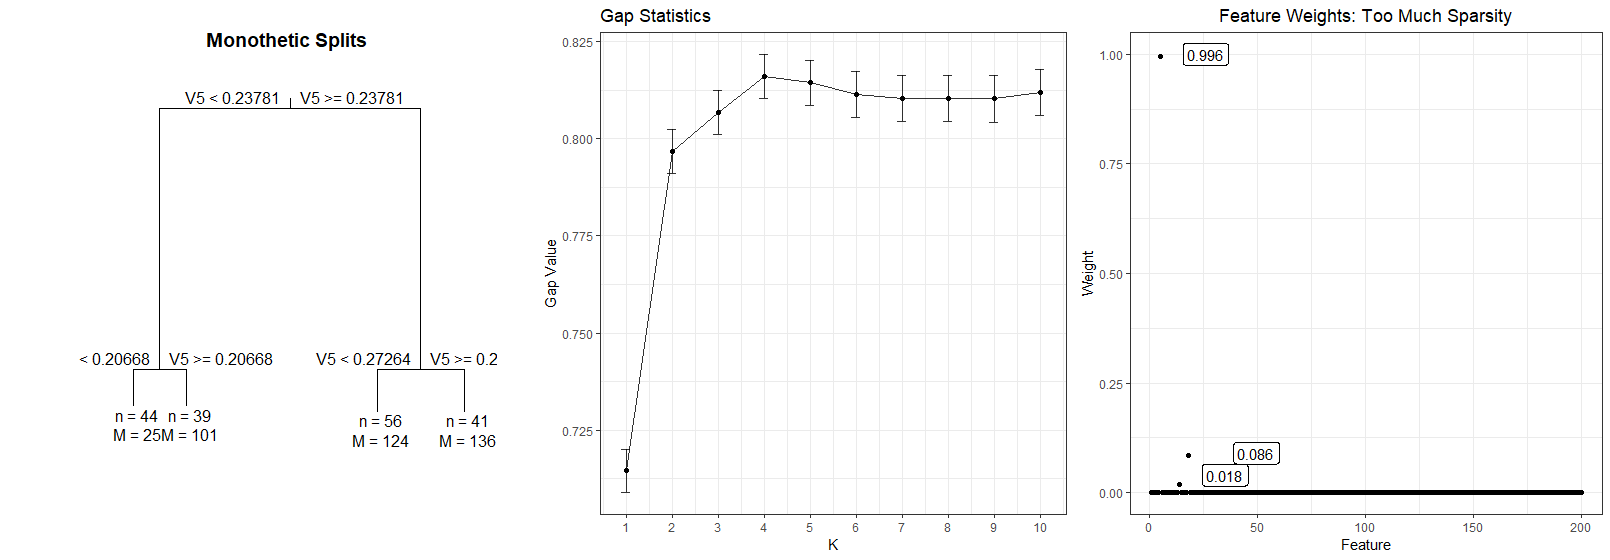
\includegraphics[width=0.9\linewidth]{TooSparseExample} \caption{Monothetic bipartitions, gap statistic values, and feature weights for too-sparse scenario.}\label{fig:ExTooSparse}
\end{figure}

This underscores the need to get both tuning parameters right - and
because monothetic clustering makes bipartitions on a single feature at
a time, an overly sparse solution may prove more punitive than in a
polythetic situation where other non-zero features may get used in the
cluster definitions.

Various methods exist, including the Elbow method (see Everitt, 2011),
or the average silhouette statistic (Rousseuw, 1987) and Caliński and
Harabasz's Pseudo F statsitic (1974). These methods can be used to
identify the optimal number of clusters as long as \(K \geq 2\) but do
not inform the critical question of whether clustering is reasonable or
not (i.e., does \(K = 1\)). Tibshirani, Hastie and Walther (2003) define
the Gap statistic as traditionally defined for generating the optimal
number of clusters for k-means and hierarchical clustering.

Indeed, no method for identifying \(K\) is perfect; the Gap statistic
was found by Sugar and James (2003) to fail to detect a clear
four-cluster solution generated from distinct exponential distributions,
and Dudoit and Fridlyand (2002) note that the Gap statistic has been
found to overestimate the optimal number of clusters in some
applications. Numerous improvements have been proposed to the Gap
statistic, including the Weighted Gap method of Yan and Ye (2007) that
leverages a weighted verson of the within-cluster sum of errors as the
intra-cluster dispersion measure.

In their implementation of sparse hierarchical clustering, Tibshirani
and Witten (2011) use a modified gap statistic based on permuted data to
generate a tuning parameter for \(s\) only, with \(K\) fixed. Thus, the
solution presented by Witten and Tibshirani does not account for the
problem of having uncertainty in the number of clusters. Some work has
been done on tackling that problem in the case of Sparse K-Means.
Brodinova et al (2019) devised a method to tune both parameters
simultaneously and suggest that choosing either \(s\) or \(k\) first
will lead to incorrect group identification. They propose using a
modified gap statistic \(Gap_{s,k}\) that can take both \(k\) and \(s\)
into account, and weights the observations as well as the features to
reduce the potential impact of outliers.

\[Gap_{s,k} = E^*\{log(W_k)\} - log(W_k)\]

This simultaneous exploration of tuning can then be presented in plots
of the gap statistic shown varying either across \(k\) with different
lines used for varying values of \(s\), or vice-versa. There are various
rules for identifying the optimal gap value. In In our setting, we find
it more natural to present the x-axis of the gap statistic to vary by
\(k\). Brodinova et al (2019) directly compare across each of the tuning
parameters as part of their simultaneous tuning process.

The optimal gap statistic can be evaluated based on a choice of several
different rules. Tishirani et al (2000) originally proposed a ``1-SE''
rule which chooses a value for \(K\) as the value such that
\(Gap(k) \geq Gap_k(k+1) - SE_k(k+1)\), i.e.~choosing typically fewer
clusters than the value that achieves the maximum gap value. Witten and
Tibshirani (2010) use a similar approach for evaluating the optimal
degree of sparsity in sparse hierarchical clustering. Additionally, it
is possible to tune for the global maximuum or first local maximum, or
to choose the value of \(k\) such that it is not smaller than the
\(Gap_k(k^*)- SE_k(k^*)\) where \(Gap_k(K^*)\) is the first local
maximum

In a now bivariate setting, we have to consider \(Gap_{s,k}\) instead of
simply \(Gap_{k}\). These rules must be extended to consider both
comparing within a given \(s\) value (and across a grid of reasonable
values for \(K\) as well as across them. Brodinova et al (2019) first
choose the optimal \(s\) value based on a modified 1-SE rule based on
both the \(s\) and \(k\) values where \(Gap_{s,k}\) is maximized.
Resulting plots can be arranged so that \(Gap_{s,k}\) varies across an
x-axis for \(K\), with various lines representing the \(s\) values, or
vice-versa.

\hypertarget{simulations-sparse-vs.-non-sparse-monothetic-clustering}{%
\section{Simulations: Sparse vs.~Non-Sparse Monothetic
Clustering}\label{simulations-sparse-vs.-non-sparse-monothetic-clustering}}

\hypertarget{simulation-1-choosing-tuning-parameters}{%
\subsection{Simulation 1: Choosing Tuning
Parameters}\label{simulation-1-choosing-tuning-parameters}}

We test the method for sparse monothetic clustering on various simulated
datasets. Similar in setting to the simulations of Witten and
Tibshirani, we simulate 4 equally-sized groups with \(n = 20\),
\(p = 100\), of which only \(20\) vary across the groups. Like the
simulations used by Witten and Tibshirani for sparcl (2010), the data
matrix \(X_s\) of simulated data is technically high-dimensional, given
that it has dimension \(80 x 100\). We extend to a more extreme case of
high-dimensional data in the next set of simulations.

Rather than taking the approach of trying to optimize S or K
individually, we instead adopt the simultaneous approach of Brodinova et
al (2019). We can consider utilizing several different rules for
choosing the optimal Gap statistic value. The first local maximum,
global maximum methods tend to pick the correct number of clusters
correctly regardless of value of S; the First SE method of Maechler
(2012), Global SE method of Dudoit and Fridlyand (2002), and
Tibshirani's original 1-SE proposition (2001) all appear to pick either
2 or 3 clusters more often than the correct value (at least across
values of S).

The goals of this simulation are twofold: First, we wish to empirically
compare rules for tuning the multi-parameter gap statistic to recommend
a method for simultaneous tuning. Additionally, we seek to highlight
that properly-tuned sparse monothetic clustering will provide better
grouping as compared to monothetic clustering on entire set of features.

Figure XX shows the gap statistic values for both tuning parameters,
presented in the left-hand panel with the x-axis represnting the \(K\)
values, and in the right-hand panel varying over the \(s\) values. We
find that the latter plot style better informs the initial question of
whether clustering should be performed or not, because the 1-cluster
solution is presented as a line across all potential sparsity parameter
values. In the example in Figure XX, it is clear that on simulated data
with clear structure, there is evidence of more than a single cluster.

\begin{figure}
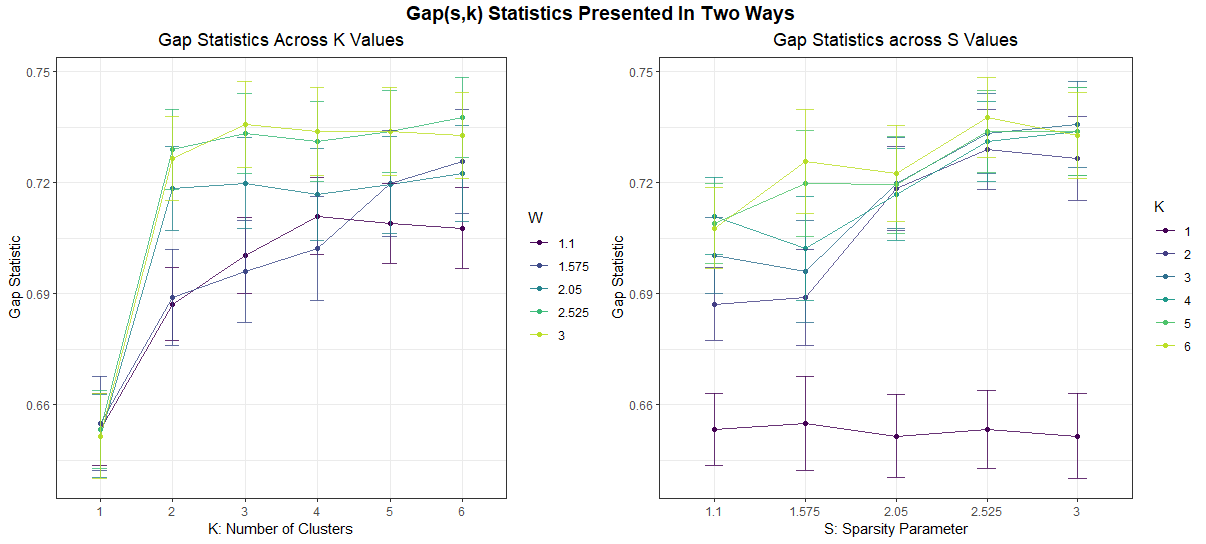
\includegraphics[width=0.9\linewidth]{Gap2Ways} \caption{Gap Statistics across s, k visualized in two methosds.}\label{fig:GapPlot1}
\end{figure}

Across each of the 10 simulations, the optimal \(s\),\(k\) can be
computed based on multivariate extensions to the rules previously
overviewed.

\begin{itemize}
\tightlist
\item
  Global Max: Choose \(S\),\(k\) such that overall gap value is
  optimized.
\item
  First Max: Gives the location of the first local maximum (given that
  Gap values are sorted by \(s\) and \(k\)).
\item
  Tibshirani: Choose the smallest values of \(s\) and \(k\) such that
  \(Gap_{s,k}(s,k) \geq Gap_{s,k}(s+s*, k+1)\) where \(s^*\) is one-unit
  step on the (either fine or course) grid of evaluated values of \(s\).
\item
  First SE Max: Proposed by Maechler (2012), chooses the smallest gap
  such that it is not less than the first local maximum minus its
  associated standard error, choosing
  \(Gap_{s,k}(s,k) \geq localmax(Gap_{s,k}(s,k)) - SE(localmax(Gap_{s,k}(s,k)))\)
\item
  Global SE: Following Dudoit and Fridlyand (2002), chooses the smallest
  \(Gap_{s,k}(s,k) \geq max(Gap_{s,k}(s,k)) - SE(max(Gap_{s,k}(s,k)))\)
\end{itemize}

The number of clusters selected by each of the rules is given as
follows.

\begin{figure}
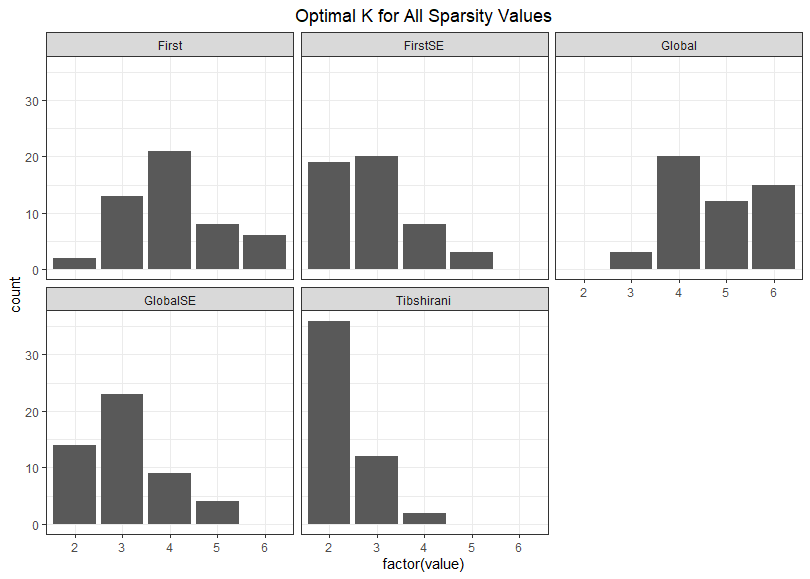
\includegraphics[width=0.9\linewidth]{OptimalKPlot} \caption{Optimal Number of Clusters Chosen by Each of the Rules across 10 simulations.}\label{fig:NumClust}
\end{figure}

The feature weights for the gap-tuned sparse clusterings are shown in
Figure XX. In most cases, the choice of weights is appropriate as we
would expect the first 20 features to have non-zero weights and the last
80 noise features should be set to 0.

\begin{figure}
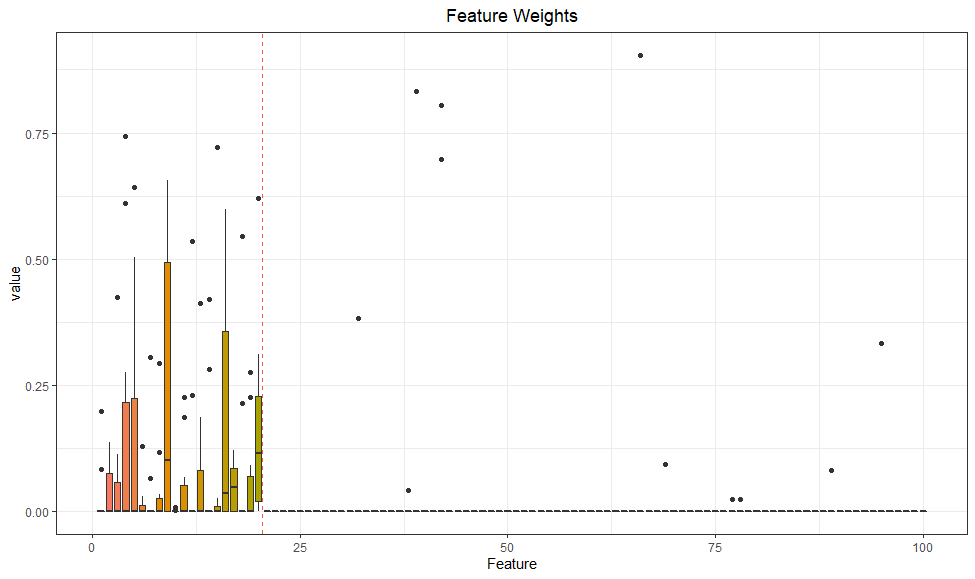
\includegraphics[width=0.9\linewidth]{Feature_Weights_425sims} \caption{Weights of features from gap-tuned sparse monothetic clustering.}\label{fig:FeatureWeights}
\end{figure}

\hypertarget{simulation-2-comparison-with-other-methods}{%
\subsection{Simulation 2: Comparison with Other
Methods}\label{simulation-2-comparison-with-other-methods}}

We consider a second set of simulations, where we assess the quality of
resulting clusterings across several methods. We compare the resulting
Rand Index metrics for each of the methods.

The data are simulated to have

\begin{itemize}
\tightlist
\item
  What rule used for ``optimal'' tuning?
\item
\end{itemize}

Figure XX shows a parallel coordinate plot of the simulated data with
noise features and the first 20 features shown as varying across each of
the 6 groups.

\begin{figure}
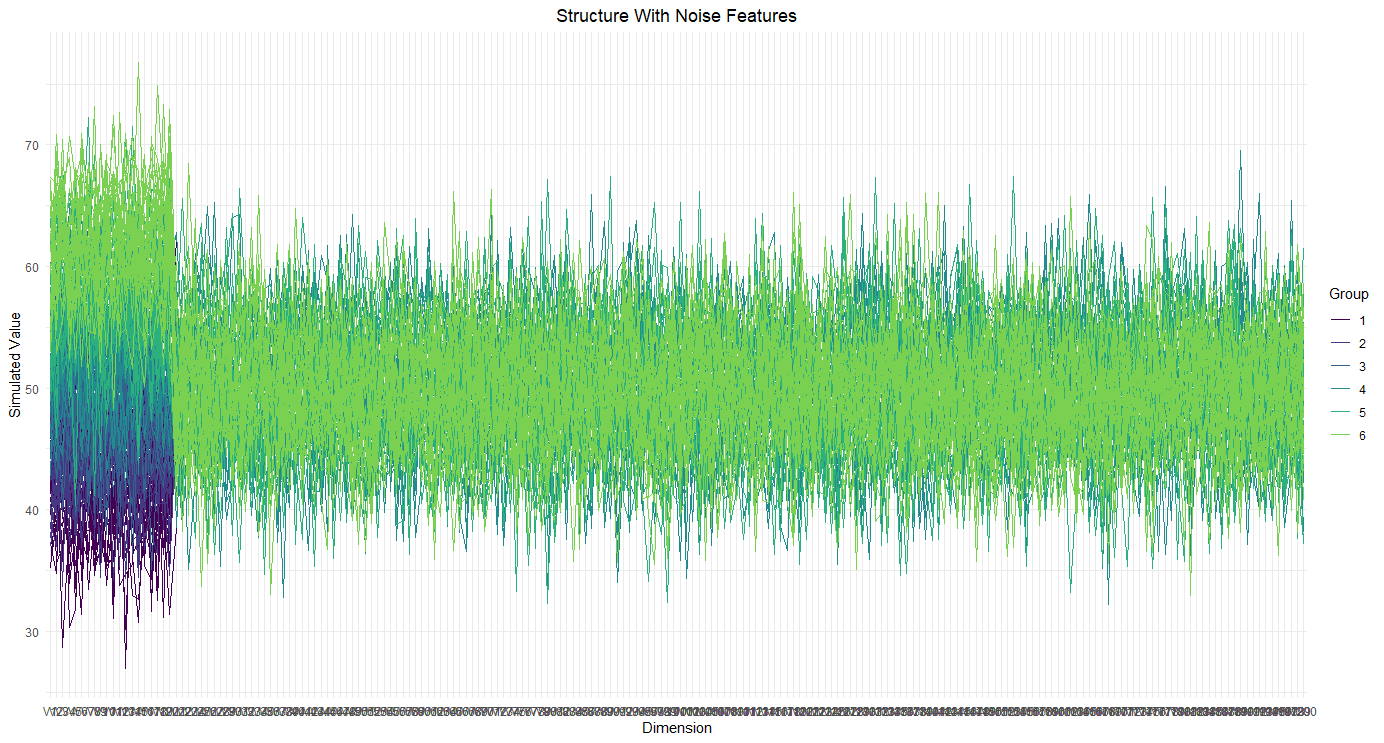
\includegraphics[width=0.9\linewidth]{SimulatedRealization} \caption{Realization of the simulated datasets.}\label{fig:SimulationRealized}
\end{figure}

\begin{tabular}{ |p{3cm} |p{3cm}|p{3cm}|p{3cm}|p{3.5cm}|  }
 \hline
 \multicolumn{5}{|c|}{Table X: Rand Index by Clustering Method} \\
 \hline
% ~ & Non-Sparse MonoClust & PMD-Based Sparse MonoClust & COSA-based Sparse MC & Oracle-Based Sparse MC \\
Simulation & Method & Rand & SE(Rand) & Mean Nonzero Coef \\
 \hline
Small Sim & Non-Sparse MC  & bbb    & ccc &   0 \\
~ & Sparse MC & z & z & z \\
~ & Oracle MC & z & z & 20 \\
~ & Non-Sparse HC & z & z & 0 \\
~ & Sparse HC & z & z & z \\
 \hline
 Big Sim & Non-Sparse MC & z & z & 0 \\
~ & Sparse MC & z & z & z \\
~ & Oracle MC & z & z & 20 \\
~ & Non-Sparse HC & z & z & 0 \\
~ & Sparse HC & z & z & z \\
 
  \hline
\end{tabular}

Comment on the results:

\begin{itemize}
\item
  Efficacy of the sparsification procedure
\item
  efficacy of the clusterings
\item
  It's possible that the results may not be great if we ``fix'' the
  problem of picking the right number of clusters
\end{itemize}

\hypertarget{real-data-analysis}{%
\section{Real Data Analysis}\label{real-data-analysis}}

\hypertarget{penguins-with-added-noise-features}{%
\subsection{Penguins? (with added noise
features?)}\label{penguins-with-added-noise-features}}

\hypertarget{carnegie-classification-dataset}{%
\subsection{Carnegie Classification
Dataset}\label{carnegie-classification-dataset}}

\hypertarget{golf-data}{%
\subsection{Golf Data?}\label{golf-data}}

\hypertarget{results}{%
\section{Results}\label{results}}

\hypertarget{computational-gains}{%
\subsection{Computational Gains}\label{computational-gains}}

Inducing sparsity prior to using monothetic clustering allows for
potential gains in compuatational efficiency, an additional benefit in
addition to providing a more interpretable set of bipartitions and
potentially more accurate clustering. The computational complexity of
monothetic clustering on numeric data is \(o(Kpn(log(n) + p))\) where
\(K\) is the number of clusters of the finest partition, \(p\) the
number of features, and \(n\) the number of objects (Chavent, 2007).
Compared to agglomerative hierarchical clustering methods with Ward's
method, which can be implemented with complexity \(o(n^2)\) (see
MacQuitty, 1966; Chavent, 2007).

The reduction in features used from \(n\) to \(n* = n-q\) features
reduces the computational complexity of the sparse hierarchical
clustering faster than it does for sparse monothetic clustering, but in
either case, a sparse solution has the potential to greatly reduce the
computational load. Much of this is explained by the simple fact that by
reducing the number of features input to the monothetic clutering
algorithm, the number of bipartitions necessary to explore at each split
is potentially substantively reduced.

Note that at least when comparing sparse monothetic clustering to other
forms of sparse hierarchical clustering, the time to calculate the
\(nxn\) dissimilarity matrix should be considered; however, it is worth
considering that our implementation calculates this twice - both in the
step to calculate the weights and sparse reweighted
dissimilarity/distance matrix, and again in the actual calculation of
the monothetic clustering (on the new dissimilarity/distance matrix).

\hypertarget{discussion}{%
\section{Discussion}\label{discussion}}

We have proposed a method for improving results in monothetic clustering
using a two-step algorithm: first, selecting relevant features via a
sparsification method to generate a set of weights \(w\) and re-weighted
dissimilarity matrix \(u\), and then to perform monothetic clustering on
that reweighted data. This extends the framework of sparse hierarchical
clustering to the divisive monothetic clustering method of Chavent
(1998). Results indicate that, at least in some cases, the bipartitions
made on sparse input data will be more interpretable and lead to better
clustering results when the true class labels are known.

Because this method relies on Witten and Tibshirani's penalized matrix
decomposition to re-weight the input data matrix, the same computational
constraints are a potential consideration. If either \(n\) or \(p\) are
very large, this method may perform slowly; indeed, by comparison to
sparse hierarchical clustering proposed by Witten and Tibshirani, sparse
monothetic may be more problematic because monothetic clustering is
typically slower than traditional hierarchical clustering.

\hypertarget{external-data-features}{%
\subsection{External Data Features}\label{external-data-features}}

Not all data used to inform the monothetic clusterings should be used as
candidates for bipartitions. Some variables may be more difficult or
expensive to obtain than others. In some settings, it may be useful to
consider temporal variables such as year or month as external features
that could be useful in explaining clusters. Sparsity may provide an
automated path to constrain the feature set used in monothetic
clustering, informing better techniques for future data collection that
are data-driven, or used in combination with external features. Chavent
also discusses using monothetic clustering with geographical constraints
(2008) - some such features may be reasonable choices in a constrained
clustering scenario.

\hypertarget{future-work-and-extensions}{%
\subsection{Future Work and
Extensions}\label{future-work-and-extensions}}

This method currently considers only quantitative variables. Tran (2019)
points out that categorical features with many categories, or mixtures
of data that include both categorical and quantitative features, can
lead to computational difficulty in searching for best splits. Chavent
(2015) attempts to tackle this problem with Divclus-T method on
non-sparse data; however, obtaining the reweighted sparse data matrix to
use as input is not a trivial problem. It does, however, represent a
useful avenue for direct extensions to this work, perhaps extending work
related to the Grouped Lasso (Choi, Park, \& Seo, 2012).

Additionally, it would be useful to identify a framework for a one-step
solution to both induce sparsity and generate clusters simultaneously.
The two-step framework of Witten and Tibshirani provides a useful tool
for extending sparsity to various methods, but a more natural way to
select features and generate clusters may be found in Bayesian methods
such as mixture modeling. Alternatively, different methods than the PMD
or COSA-based method for obtaining the sparse input matrix to the
monothetic clustering may provide alternate forms of
regularization/feature selection that could be worth investigating in
the future.

Further documents, test versions of scripts, relevant datasets, and
other details can be found at Github: {[}\emph{insert link here}{]}

\hypertarget{appendix}{%
\section{Appendix}\label{appendix}}

An example of

\hypertarget{clear-structure-with-noise-features}{%
\subsection{Clear Structure With Noise
Features}\label{clear-structure-with-noise-features}}

The algorithm that I employed to try to figure out the number of
clusters and optimal sparsity is as follows. I considered a fine grid of
tuning parameter values and numbers of clusters.

\begin{itemize}
\tightlist
\item
  Fix \(s\): Given a choice of sparsity,
\item
  Calculate the Hierarchical Clustering and obtain U and dendrogram
\item
  Then, fix \(k\), the number of clusters. For \(k\), I calculate the
  \(w_k\) value based on the above function
\item
  Iterate through each of the \(k\) values and store each \(w_k\) in a
  vector
\item
  Now, generate a permuted dataset that feeds into the Hierarchical
  Clustering. Re-obtain U and new dendrogram
\item
  Fix \(k\) again and calculate \(w_k\), iterating through each \(k\).
  Store as vector and combine into a matrix with a column per
  permutation.
\item
  Now, calculate the gap statistics using the equal-weight formula and
  generate SE's
\item
  Store gap statistics, SE's, etc. in a list that is updated for each
  value of \(s\).
\end{itemize}

\hypertarget{increasing-noise}{%
\subsection{Increasing Noise}\label{increasing-noise}}

\hypertarget{increasing-number-of-groups}{%
\subsection{Increasing Number of
Groups}\label{increasing-number-of-groups}}

\emph{Table with each row CER/Rand index, percentage that get K right}

\begin{tabular}{ |p{3cm}|p{3cm}|p{3cm}|p{3cm}|  }
 \hline
 \multicolumn{4}{|c|}{Rand Index by Clustering Method} \\
 \hline
 Non-Sparse & PMD-Based Sparse MonoClust & COSA-based Sparse MC & Oracle-Based Sparse MC \\
 \hline
 Aaa   & bbb    & ccc &   ddd \\
 Aland Islands&   AX  & ALA   &248\\

 \hline
\end{tabular}

\end{document}
